\documentclass[12pt]{article}

% Packages
\usepackage[margin=1in]{geometry}
\usepackage{booktabs}
\usepackage{dcolumn}
\usepackage{amsmath}
\usepackage{graphicx}
\usepackage{caption}
\usepackage{float}
\usepackage{setspace}
\usepackage{hyperref}
\usepackage{natbib}
\usepackage{enumitem}

% Title Information
\title{Research Methods II: Homework 3}
\author{UNI: XW3000}
\date{\today}
\setlength{\parindent}{0pt}

\begin{document}
\maketitle

\section{Import Data}

The csv data is imported and labeled accordingly. 

\section{Balance Table}

Through Balance Table analysis, we assess whether there are systematic differences between ranked and unranked institutions. The covariates of interest include academic quality, athletic quality, and proximity to major markets. We employ Welch's t-tests to account for potential differences in variance between groups. Table \ref{tab:balance} presents the balance analysis comparing ranked and unranked colleges.

\begin{table}[H]
    \begin{center} 
    \caption{\textbf{Balance Table: Ranked vs. Unranked Colleges}}
    \label{tab:balance}
    \begin{tabular}{l*{6}{c}}
                    &    Unranked&      Ranked&  Difference   \\
\hline
Academic Quality    &       0.515&       0.466&       0.049   \\
Athletic Quality    &       0.424&       0.551&      -0.127** \\
Near Big Market     &       0.360&       0.700&      -0.340***\\
\multicolumn{6}{p{0.6\linewidth}}{\small *** p$<$0.01, ** p$<$0.05, * p$<$0.1} \\
\\
\multicolumn{6}{p{0.6\linewidth}}{\small \textbf{Notes:} This table presents the balance analysis comparing ranked and unranked colleges. The null hypothesis is that the difference in means between ranked and unranked colleges for each characteristic is zero ($H_0: \mu_1 - \mu_2 = 0$).} \\
\end{tabular}

    \end{center}
\end{table}

From Table 1, we reject the null hypothesis that there is no difference in \textit{athletic quality} and \textit{proximity to major markets} between the ranked and un-ranked institutions. Although we fail to reject the null for \textit{academic quality}, the treatment and control groups do \textbf{not} appear similar. The differences exist in their athletic quality and proximity to major markets.

\section{Comments on Propensity Score Matching (PSM)}

Propensity score matching methods are more credible when we are able to use all variables that potentially influence the treatment assignment. In our context, we unfortunately do not have access to all variables that could impact whether a college is ranked or not ranked as having a top basketball program. This limitation thus undermines the credibility of propensity score methods in studying the causal effect of being ranked on alumni donations the following year. 

\section{PSM Model}

We build a logistic regression model predicting ranking status using three key institutional characteristics: academic quality, athletic quality, and proximity to major markets. Specifically:
\begin{equation}
\log\left(\frac{P(Ranked = 1)}{1-P(Ranked = 1)}\right) = \beta_0 + \beta_1 AcademicQuality + \beta_2 AthleticQuality + \beta_3 NearBigMarket
\end{equation}

\subsection{Logistic Regression Results}

Table \ref{tab:logit} presents the logistic regression results.

\begin{table}[H]
    \centering
    \caption{Logistic Regression Results: Predicting College Rankings}
    \label{tab:logit}
    \begin{tabular}{l*{2}{c}}
\hline\hline
                    &\multicolumn{1}{c}{(1)}\\
                    &\multicolumn{1}{c}{Ranked }\\
                    & Coefficient         \\
\hline
Ranked &                     \\
Academic Quality    &      -0.884         \\
                    &       (0.780)         \\
Athletic Quality    &       1.964\sym{**} \\
                    &       (0.806)         \\
Near Big Market     &       1.615\sym{***}\\
                    &       (0.459)         \\
Constant            &      -1.378\sym{**} \\
                    &       (0.645)         \\
\hline
Observations        &         100         \\
Pseudo R-squared    &       0.141         \\
\hline\hline
\multicolumn{2}{p{0.6\linewidth}}{\small *** p$<$0.01, ** p$<$0.05, * p$<$0.1} \\
\multicolumn{2}{p{0.6\linewidth}}{\small \textbf{Notes:} This table presents coefficient estimates from a logistic regression predicting college ranking status. Coefficients represent log odds. Standard errors are shown in parentheses. } \\
\end{tabular}



\end{table}

As shwon in Table 2, \textit{Athletic Quality} and \textit{Near Big Market} are statistically significant predictors of ranking status. A one-unit increase in athletic quality is associated with a 1.964 increase in the log odds of being ranked (odds ratio = $e^{1.964} = 7.13$), while being near a big market increases the log odds by 1.615 (odds ratio = $e^{1.615} = 5.03$). Consistent with Balance Table analysis, \testit{Academic Quality} shows a negative but statistically insignificant relationship with ranking status.

\subsection{Estimated Propensity Scores}

Using estimated coefficients in Table 2, I calculated propensity scores for each institution. 

The Stata command \texttt{predict propensity\_score, pr} generates the predicted probabilities. Please see HW3-Stata.do for more details.

\section{Distribution of Propensity Scores}
Figure \ref{fig:prop_dist} shows the distribution of propensity scores across ranked and unranked institutions. 

\begin{figure}[H]
    \centering
    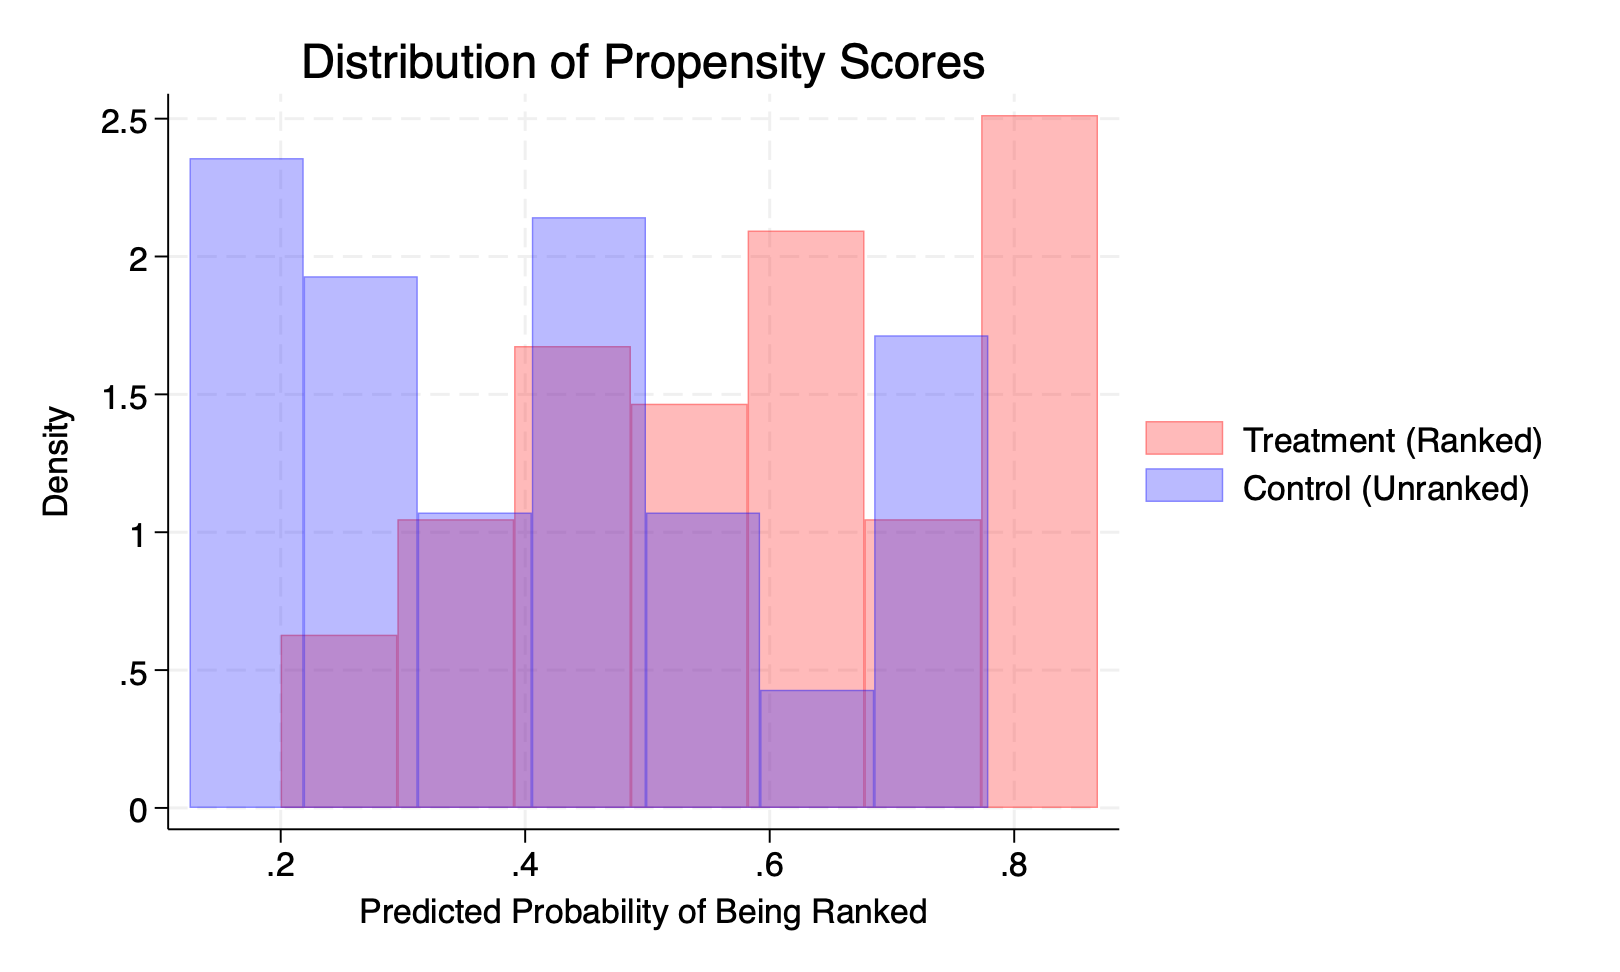
\includegraphics[width=0.8\textwidth]{propensity_distribution.png}
    \caption{\textbf{Distribution of Propensity Scores by Ranking Status}}
    \label{fig:prop_dist}
\end{figure}

\section{Group Observations}

We sort observations by their propensity scores and create blocks of ten observations each. This blocking helps control for underlying differences between ranked and unranked colleges by comparing institutions with similar probabilities of being ranked.

\section{Treatment Effect with Block Fixed Effects}

To estimate the causal effect of rankings on alumni donations while accounting for selection, we implement a block fixed effects approach. 

The empirical specification is:

\begin{equation}
AlumniDonations_i = \beta_0 + \beta_1 Ranked_i + \beta_2 X_i + \gamma_b + \epsilon_i
\end{equation}

where $X_i$ represents the vector of covariates (academic quality, athletic quality, and market proximity), and $\gamma_b$ represents block fixed effects. Table \ref{tab:block_effects} on next page presents the results.\\

The inclusion of block fixed effects helps address selection bias by ensuring comparison of ranked and unranked colleges with similar propensity scores and reducing bias from non-random selection into rankings.\\

The coefficient on Ranked ($\beta_1$) represents the estimated causal effect of rankings on alumni donations, controlling for both observable characteristics and unobservable factors that might be correlated within propensity score blocks. The effect of being ranked on the alumni donation of the following year is estimated to be 500.47 (thousands of dollars), comparing to institutions not ranked, controlling for academic quality, athletic quality, proximity to big market, and the propensity score of being ranked.


\begin{table}[H]
    \centering
    \caption{\textbf{Effect of Rankings on Alumni Donations with Block Fixed Effects}}
    \label{tab:block_effects}
    \begin{tabular}{l*{4}{c}}
\hline\hline
                    &\multicolumn{4}{c}{(1)}\\
                    &\multicolumn{4}{c}{Alumni Donations}\\
\hline
Ranked              &     500.479\sym{***}\\
                    &       (0.234)         \\
Academic Quality    &     100.198\sym{***}\\
                    &       (0.752)        \\
Athletic Quality    &      49.718\sym{***}\\
                    &       (1.661)         \\
Near Big Market     &     999.487\sym{***}\\
                    &       (1.319)         \\
Propensity Score Block=1&      -0.242         \\
                    &       (0.859)         \\
Propensity Score Block=2&      -0.223         \\
                    &       (0.978)        \\
Propensity Score Block=3&       0.709         \\
                    &       (1.144)         \\
Propensity Score Block=4&       0.758         \\
                    &       (1.288)         \\
Propensity Score Block=5&       0.622         \\
                    &       (1.467)         \\
(...)\\
Propensity Score Block=20&       3.455         \\
                    &       (4.974)         \\
Propensity Score Block=21&       3.846         \\
                    &       (5.347)         \\
Propensity Score Block=22&       4.334         \\
                    &       (5.641)         \\
Propensity Score Block=23&       4.275         \\
                    &       (6.091)         \\
Propensity Score Block=24&       4.276         \\
                    &       (6.536)         \\
Propensity Score Block=25&       5.262         \\
                    &       (6.773)         \\
Constant            &      -0.137         \\
                    &       (0.933)         \\
\hline
Observations        &         100         \\
Adjusted R-squared  &       1.000         \\
F-statistic         &  1278547.74         \\
\hline\hline
\multicolumn{4}{p{0.6\linewidth}}{\small *** p$<$0.01, ** p$<$0.05, * p$<$0.1} \\
\multicolumn{4}{p{0.6\linewidth}}{\footnotesize This table presents OLS estimates of the effect of college rankings on alumni donations. Block fixed effects are included to control for propensity score quartiles. Standard errors are in parentheses. Blocks are created by grouping every 4 observations based on predicted probability of being ranked from the propensity score model.}\\
\end{tabular}
\end{table}


\end{document}